\section{Open-loop planning via n-steps ahead predictions}
\label{sec:open_loop_planning}

The proposed approach requires the presence of $H+1$ versions of the matrix $\bP$ at each grid point. One of these versions is initialized with $\bar{\bP}_0$, while the others represent the evolution of matrices that were initialized at previous grid points, from 1 to $H$ steps earlier. This ensures that at each step it is possible to find a covariance matrix evolved for $H$ steps and use it to robustify the constraint. 
To adapt the problem, it is necessary to modify equations (\ref{eq:DOCPdP}) and (\ref{eq:DOCPconstraints}). In this case,  (\ref{eq:DOCPdP}) collects $H$ collocation and continuity equations and an initialization equation, while (\ref{eq:DOCPconstraints}) takes as input the most propagated version of the covariance matrix at the k-th step, here named $\bP^H_k$. The new formulation is reported:
\begin{alignat}{3}
\bzero       = & \; \bPsiP_k(\bmu_k,\bxi_k, \bu_k, \bP_{k-1}^{j-1},\bP_k^j,\bSi_k^j,\bz_k),
& \quad & k = 1,\ldots, N; \; j=0,\ldots,H \label{eq:DOCPdPopenloop} \\
0            \geq & \; h_i(\bmu_k, \bu_k, \bz_k) + \be_i(\bmu_k, \bu_k, \bP_k^j, \bz_k),
& \quad & k = 1,\ldots, N;\; i \in \calI \label{eq:DOCPconstraintsopenloop}
\end{alignat}
This process is illustrated in Figure \ref{fig:DOCPgrid}, where the dashed rectangle represent the $k$-th step at which the constraints are being formulated. At each grid point, two versions of the covariance matrix are highlighted: $\bP^0_k$ (red node), which is the version to be initialized, and $\bP^H_k$ (green node), which is the most propagated version used to formulate the robust constraints in equation (\ref{eq:DOCPconstraints}).

\begin{figure}
	\centering
	\begin{tikzpicture}[%
		smallnode/.style={%
			circle, draw, minimum size=3mm, inner sep=0pt
		},
		r_smallnode/.style={%
			circle, draw, minimum size=3mm, inner sep=0pt, red
		},
		g_smallnode/.style={%
			circle, draw, minimum size=3mm, inner sep=0pt, mygreen
		},
		every path/.style={->, thick},
		x=1.5cm, y=1.5cm
		]
		
		\newcommand{\Plab}[2]{\bP^{#2}_{#1}}
		\definecolor{mygreen}{RGB}{0 150 0}
		
		% Nodes
		% First row
		\node[smallnode, label={[label distance=-2pt]above:\protect\(\Plab{k-2}{H-2}\)}] (Pk-2H-2) at (1,0) {};
		\node[smallnode, label={[label distance=-2pt]above:\(\Plab{k-1}{H-1}\)}] (Pk-1H-1) at (2,0) {};
		\node[g_smallnode, label={[label distance=-2pt]above:\(\Plab{k}{H}\)}] (PkH) at (3,0) {};
		\node[r_smallnode, label={[label distance=-2pt]above:\(\Plab{k+1}{0}\)}] (Pk+10) at (4,0) {};
		\node[smallnode, label={[label distance=-2pt]above:\(\Plab{k+2}{1}\)}] (Pk+21) at (5,0) {};
		
		% Second row
		\node[smallnode, label={[label distance=-2pt]above:\(\Plab{k-2}{H-3}\)}] (Pk-2H-3) at (1,1) {};
		\node[smallnode, label={[label distance=-2pt]above:\(\Plab{k-1}{H-2}\)}] (Pk-1H-2) at (2,1) {};
		\node[smallnode, label={[label distance=-2pt]above:\(\Plab{k}{H-1}\)}] (PkH-1) at (3,1) {};
		\node[g_smallnode, label={[label distance=-2pt]above:\(\Plab{k+1}{H}\)}] (Pk+1H) at (4,1) {};
		\node[r_smallnode, label={[label distance=-2pt]above:\(\Plab{k+2}{0}\)}] (Pk+20) at (5,1) {};
		
		% dots row 
		\node[label={center,rotate=90:\(\dots\)}] (dots2) at (1, 1.7) {};
		\node[label={center,rotate=90:\(\dots\)}] (dots3) at (2, 1.7) {};
		\node[label={center,rotate=90:\(\dots\)}] (dots4) at (3, 1.7) {};
		\node[label={center,rotate=90:\(\dots\)}] (dots5) at (4, 1.7) {};
		\node[label={center,rotate=90:\(\dots\)}] (dots6) at (5, 1.7) {};
		
		% Third row 
		\node[g_smallnode, label={[label distance=-2pt]above:\(\Plab{k-2}{H}\)}] (Pk-2H) at (1,2) {};
		\node[r_smallnode, label={[label distance=-2pt]above:\(\Plab{k-1}{0}\)}] (Pk-10) at (2,2) {};
		\node[smallnode, label={[label distance=-2pt]above:\(\Plab{k}{1}\)}] (Pk1) at (3,2) {};
		\node[smallnode, label={[label distance=-2pt]above:\(\Plab{k+1}{2}\)}] (Pk+12) at (4,2) {};
		\node[smallnode, label={[label distance=-2pt]above:\(\Plab{k+2}{3}\)}] (Pk+23) at (5,2) {};
		
		% Fourth row
		\node[smallnode, label={[label distance=-2pt]above:\(\Plab{k-2}{H-1}\)}] (Pk-2H-1) at (1,3) {};
		\node[g_smallnode, label={[label distance=-2pt]above:\(\Plab{k-1}{H}\)}] (Pk-1H) at (2,3) {};
		\node[r_smallnode, label={[label distance=-2pt]above:\(\Plab{k}{0}\)}] (Pk0) at (3,3) {};
		\node[smallnode, label={[label distance=-2pt]above:\(\Plab{k+1}{1}\)}] (Pk+11) at (4,3) {};
		\node[smallnode, label={[label distance=-2pt]above:\(\Plab{k+2}{2}\)}] (Pk+22) at (5,3) {};
		
		% Curved arrows
		\draw[bend left=20] (Pk-2H-2) to (Pk-1H-1);
		\draw[bend left=20] (Pk-1H-1) to (PkH);
		\draw[bend left=20] (Pk+10) to (Pk+21);
		
		\draw[bend left=20] (Pk-2H-3) to (Pk-1H-2);
		\draw[bend left=20] (Pk-1H-2) to (PkH-1);
		\draw[bend left=20] (PkH-1) to (Pk+1H);
		
		\draw[bend left=20] (Pk-10) to (Pk1);
		\draw[bend left=20] (Pk1) to (Pk+12);
		\draw[bend left=20] (Pk+12) to (Pk+23);
		
		\draw[bend left=20] (Pk-10) to (Pk1);
		\draw[bend left=20] (Pk1) to (Pk+12);
		\draw[bend left=20] (Pk+12) to (Pk+23);
		
		\draw[bend left=20] (Pk-2H-1) to (Pk-1H);
		\draw[bend left=20] (Pk0) to (Pk+11);
		\draw[bend left=20] (Pk+11) to (Pk+22);
		
		% Dashed rectangle
		\draw[dashed, thick, rounded corners] (2.6,-.25) rectangle (3.4,3.5);
		
	\end{tikzpicture}
	\caption{}
	\label{fig:DOCPgrid}
\end{figure}

\subsection{Direct Collocation}
The objective is to recast the MLTP into a Non Linear Program (NLP) using a direct orthogonal collocation approach, specifically based on Gauss-Legendre collocation points. The problem is formulated within the CasADi framework~\cite{Andersson:MPC:2019} and solved using the interior point method implemented in IPOPT~\cite{Wachter:MP:2006}. The resulting NLP can be expressed in the form:
\begin{align}
	\underset{x,v,u,z}{\textrm{minimize}}&\quad\sum_{k=1}^NL_k(x_k,v_k,u_k,z_k)\label{eqn:functional}\\
	\textrm{subject to}&\quad g_k(x_{k-1},x_k,v_k,u_k,z_k)=0,\ k=1,\ldots,N,\label{eqn:equality}\\
	&\quad h_k(x_k,u_k,z_k)\le0,\ k=1,\ldots,N.\label{eqn:inequality}
\end{align}
In Eqs.~\eqref{eqn:functional}, \eqref{eqn:equality} and \eqref{eqn:inequality}, in addition to the state and control vectors, $v_k$ and $z_k$ are included, representing the state vector at the collocation points and the algebraic quantities, respectively. The controls and the algebraic variables are approximated as piecewise constant, while the states are approximated as quadratic polynomials within each finite element. Specifically, the algebraic variables in the problem are the time steps $\nu_k$ and the lateral and vertical displacements of the Center of Mass relative to the origin of the $k$-th frame $\sref{S}$, attached to the track's centerline ($e_y$ and $e_z$). Their function is to serve as handle variables in the optimization process to promote problem sparsity.

The track centerline is represented by a curvilinear abscissa $\alpha\in[0,1]$, sampled at $N+1$ points $\alpha_0,\ldots,\alpha_N$. Each grid point is associated with a reference frame $\sref{S_k}$, whose origin lies at the corresponding point on the track centerline, as illustrated in Figure~\ref{fig:track_frames}. A more detailed description of the 3D track modeling can be found in~\cite{Bartali:Meccanica:2023}. Specifically, this representation allows us to capture track slope and banking, but it does not support non-developable track surfaces.

\begin{figure}[h]\centering
	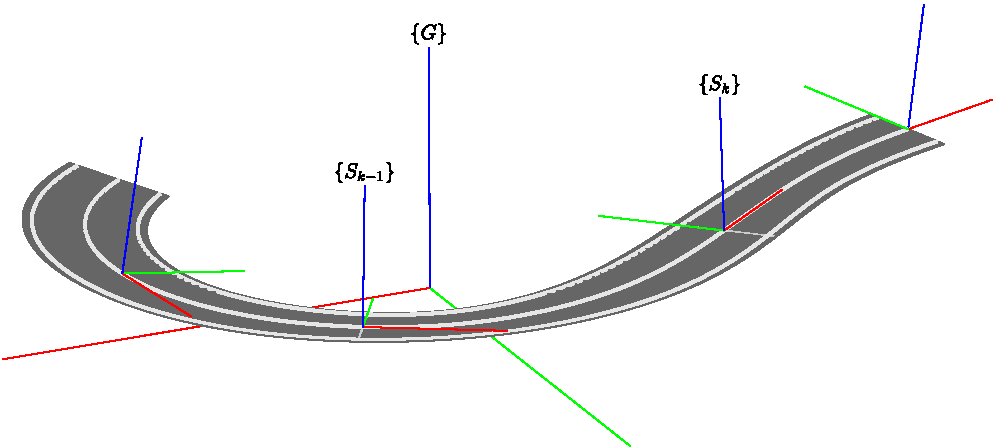
\includegraphics[width=0.8\textwidth]{Images/track_frames.pdf}
	\caption{Track frames corresponding to adjacent nodes of the grid over $\alpha$. Note that the grid points need not be equispaced. If desired, they can be chosen irregularly, so as to capture more features of the track where it is more critical (e.g. in proximity to corners) and save space where it is more regular (e.g. on the straights).}
	\label{fig:track_frames}
\end{figure}

%According the direct collocation method, the state evolution on the $k$-th element of the grid is approximated with a polynomial $p_k$. The number of collocation points depends on the degree $d$ of the polynomial chosen and their position inside the interval can be selected based on different criteria; here the Gauss-Legendre collocation points are used. The polynomial is built on the unit interval and then scaled to match the length $\nu_k$ of the relative time step.
%
%In Eq.~\eqref{eqn:equality}, besides specific constraints inserted to bias the solution towards desired behaviours, two equations are paramount. The first  one is:
%\begin{equation}\label{eqn:collocation}
%	\frac{1}{\nu_k}\frac{\partial}{\partial\tau}p_k(\tau_i)=f(v_{k,i},u_k),
%\end{equation}
%the collocation equation, that constrains the state at each collocation point to comply with the system dynamics. The second one, which is $p(1)=x_{k+1}$, ensures continuity across time intervals.

In addition to the classical collocation and continuity constraints~\cite{Domenighini:Designs:2023}, the inequalities in Eq.~\eqref{eqn:inequality} for our MLTP ensure the vehicle remains within track bounds. These include the requirement for the CoM to lie on the $yz$ plane of the frame $\sref{S_k}$, as well as power and adherence limits.

In our optimizations, the cost function at each step is expressed as follows:
\begin{equation}\label{eqn:cost}
	L_k=\nu_k^2+k_\delta(\delta_k-\delta_{k-1})^2+k_T(T_k-T_{k-1})^2+k_v x_{k,2}^2 + l_k(\ddot{q}_{hk,k},\delta_k,x_k),
\end{equation}
where the first term penalizes travel time, the second and third prevent abrupt variations of the inputs and avoid singular arcs. The quadratic penalization ensures a well-defined dependence of the Hamiltonian on the control variables, preventing indeterminate solutions. The last two serve to shape the driving behaviors according to the designer preferences.

Their primary goal is to improve the optimization landscape, ensuring that the solver is less likely trapped by undesirable local minima. As an example, the fourth term, which includes the lateral velocity $x_{k,2}$, has been included to prevent undesirable behaviors which could emerge as a result of the increased system's DoFs in combination with the simplified aerodynamic modeling adopted in this work. Some local minima could automatically be avoided by incorporating more realistic aerodynamic maps and tyre wear models. These enhancements will be explored in future works. In this context, an interesting direction is presented in~\cite{Masouleh:IEEE:2016}, where the authors introduce an aerodynamic model that explicitly accounts for the influence of suspension and vehicle configuration. This approach offers a more comprehensive representation of the aero forces and could be effectively used to refine the current aerodynamic map. By incorporating such a model, we expect not only a more physically consistent representation of the aerodynamics but also a smoother and more meaningful optimization landscape, reducing the occurrence of non-physical local minima and improving overall solution robustness.%More in details, the all steering vehicle, having the capability to steer independently with all four wheels, and considering that the aerodynamic drag only depends on the forward velocity $x_1$, could run with excessively large $\beta$ angles, even on straights paths. Even if this behavior could be appropriate in certain track sectors, is undesirable from an engineering perspective.
%In some cases, it could also be the outcome of the solver being stuck in local minima: in these events the above term helps discourage such behaviours.

In the current context, we imposed coefficient $k_v$ to be a function of the (absolute value of) track curvature $c_k$ according to Eq.~\eqref{eqn:lateral_cost}. Here, the two constant $\bar{k}_v$ and $k_c$ are selected heuristically for each track; the first increases/decreases the weight of the cost term, while the second varies the hardness of the intervention in the range $[0,1]$.
\begin{equation}\label{eqn:lateral_cost}
	k_v = \bar{k}_v(1-\tanh(k_c c_k))
\end{equation}

To ensure reproducibility, we report the values of the main penalty weights for the cost function terms used in the Siena track simulations: $k_{\delta} = 0.05$, $k_T = 0.005$, $\bar{k}_v = 0.005$, and $k_c = 100$. 

